in this chapter ...
first this, then that


\silvia{general notes: 
\\(1) need to give a name for the dataset "fertility data repository"? ivf/prn repo? ivf-repo something short that you can simply use in this section.
\\(2) also need a name for the SG that is the main object in the thesis. 
the terminology should be introduced in the intro and used consistently afterwards
\\(3) explain stakeholders, what they do (with and without the system)
\\(4) refer to components, module, function groups - not "blocks"
}

\section{Process Analysis}
\label{process-analysis}


\paragraph{Research workflow}
When doing research in the medical domain a well known workflow is often used. Nwogu \cite{nwogu} has formally described and defined this workflow for scientific reporting purposes (\ie{} writing scientific papers).
Figure \ref{fig:research-workflow} shows the simplification of this workflow, which includes problem definition, formulation of research question, definition of methods, data aquisition, data analysis, statistical analysis and conclusions. \silvia{i dont understand "outcomes" - does it mean stats? or results?}

Clinical research (\eg{} a trial) is well suited to follow this workflow, as each step can be executed in turn and data acquisition is often the most time-consuming part.
However, acquisition of new data is not always necessary,  desirable or even possible. 
\silvia{ "with the rise of cheap disk space and big data this does not have to be true" - this is not the motivation. data is valuable and needs to be reused, this is the motivation.}
Research data of high quality and trustworthiness can be preserved and re-used endlessly, upon well controlled conditions. 
This is the case of IVF-repo.

\paragraph{Research Workflow using the IVF-repo}
In the \project{} considerable time has been spend on gathering valuable data. The goal of this SG is to facilitate reuse of this data. 
There is, however, one major restriction with data sharing and re-use: medical data is (almost always) highly sensitive and must be secured. 
This imposes strong conditions for reusing the data, which needs to be taken into account by the system.


\begin{figure}[hb]
	\centering
	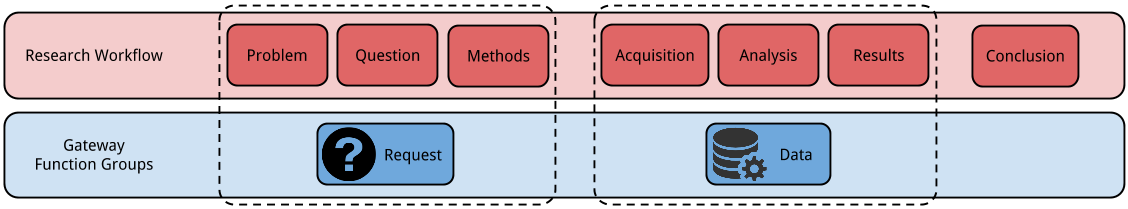
\includegraphics[width=1.0\linewidth]{images/research-workflow}
	\caption{
		This figure shows a simplification of the research workflow often used  in the medical domain (based on \cite{nwogu}).
		The workflow building blocks are mapped by the identified system function groups. Note that the data acquisition block requires execution of acquisition methods from the methods block.
	}
	\label{fig:research-workflow}
\end{figure}

\silvia{put something saying that the SG will support this process, in a case where data acquisition is actually done by consulting the XXX data repository. researchers need to find data, request it, get permission, receive the data. data managers need to keep track of all actions. 
also explain and how you move on to detail from here (functionality design)}

\section{Initial concept}

\silvia{this section is too difficult to understand, need a complete rewrite}

\silvia{i think this should be a separate section. give it a name (seed concept? seed design?) - just "seed" is not enough. There was also some study done prior to this design (interviews, study, observation).
briefly report this in 2.1. Then you can present the first design itself (fig 2.1)}

Restricting the use of data to one user is undesirable, therefore good data management has to be applied to enable re-use.
\silvia{explain where the initial idea came from (maybe this is the link with the previous part?)}
The initial idea in this project was to develop a data management system with data-centric functions, \eg{} request, upload, download, search, for .....
These are represented in figure \ref{fig:research-workflow} with the blocks `request' and `data'.
With these functions a big part of the research workflow would be supported.


\silvia{
the txt below was at the caption, but i think it should not. captions are used to explain the figure - nothing else. generic stuff goes to the text body:
External services such as .. are provided ?? and outside of the scope of this paper.
Two direct users and several external users are planned each with their specific set of functions.
		Data listed is either available at initialisation of the system or is generated during execution.
}
		
\begin{figure}[t]
	\centering
	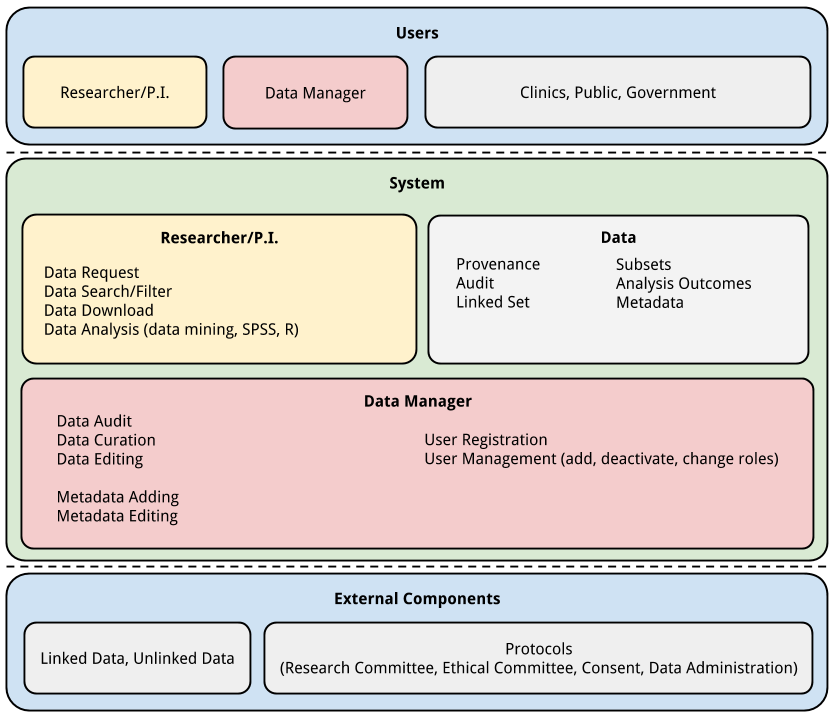
\includegraphics[width=1.0\linewidth]{images/brainstorm-before}
	\caption{
		Initial concept for the \ivfsystem{}, encompassing data and user management. 
		The system offers different sets of fuctions for three user roles (a,b,c) indicated by colors. 
		External services provide data according to regulations.
	}
	\label{fig:brainstorm-before}
\end{figure}

Figure \ref{fig:brainstorm-before} describes the full view of the seed. The function groups are expanded into: users, external services, data, and functions.
The external services provide ...
They influence the system but are outside of the scope of this paper.
This means that data and protocols (necessary for lawful execution of the system) 
are already provide by these external systems, and ???.
From the provided data, unlinked data is \project{} data split into clinics and PRN, where linked data are the matched rows from both.
Projected direct users are researchers and data managers.
Furthermore, external parties (clinics, public, government) might be interested in statistics of the system and its data, \eg{} aggregated and anonymised analysis outcomes.

Functions for each of the user roles encompass data management and user management.
Data functions meaning mutations of the raw \project{} data, where metadata is metadata of this raw data. \silvia{need to explain in intro what is data, metadata in general and in the context of this project}
The data block refers to data being stored in the system at initialisation and during execution.
The linked set (\ie{} raw data) is an initialisation input of the system.
Other items are generated during execution, \eg{} subsets are created after a data request is granted which also results in provenance data, etc.